\chapter{INTRODUCTION (WIP)}

\sepfootnotecontent{fn:path-of-exile}{Path of Exile (Grinding Gear Games, 2013). Computer Game. Microsoft Windows.}

\sepfootnotecontent{fn:diablo}{Diablo (Blizzard Entertainment, 1996). Computer Game. Microsoft Windows.}

\sepfootnotecontent{fn:dark-souls}{Dark Souls (FromSoftware, 2011). Video Game. PlayStation 3, Xbox 360, Microsoft Windows, PlayStation 4, Xbox One, Nintendo Switch, PlayStation 5.}

\sepfootnotecontent{fn:hack-and-slash}{Footnote: What are Hack and Slash Games}

\sepfootnotecontent{fn:checkpoints}{Footnote: What are Checkpoints}

\sepfootnotecontent{fn:boss-fights}{Footnote: What are boss fights}

\sepfootnotecontent{fn:mario-kart}{Footnote: What is Mario Kart}

\sepfootnotecontent{fn:half-life}{Footnote: What is Half-Life}

% ==========================================================
% About the PROBLEM
% ==========================================================

% Game Designers have to decide between large audience or niche
% For broad audience, lean towards casual players with well known features & trends
% For niche games, explore new features & create complex systems
Game Designers are often riddled by the trade off of either appealing to the largest audience possible or entertaining the preferences of a niche. When creating games for a broad audience, game designers lean towards the preferences of casual players, using predefined and well-known features to take advantage of popular trends in a game genre. When creating niche games, designers often express more freedom, exploring new features, mixing older ones and creating complex systems that are well received by the target audience. This can be seen in \emph{Path of Exile}\sepfootnote{fn:path-of-exile}, which uses mechanics previously explored by predecessor games such as \emph{Diablo}\sepfootnote{fn:diablo} and innovates by combining new features with what was already proven to be successful.

% Making game for a niche can strengthen it's core characteristics, vision, aesthetics
% One of the best examples for this is Dark Souls
Tailoring a game to a specific niche during the conceptual phase of development is a valid approach to solidifying its core vision, mechanics and aesthetics, as having well defined delimiters to design decisions simplifies the conception of new systems and promotes a focused and iterative improvement process. One of the most notable examples of successful games that were originally targeted for a niche audience is \emph{Dark Souls}\sepfootnote{fn:dark-souls}, a challenging \emph{Hack and Slash}\sepfootnote{fn:hack-and-slash} RPG (Role-Playing Game) which is considered one of the most influential games of all time and  the origin of the \emph{Souls-like} game genre \cite{BOOK_DarkSoulsBeyondTheGrave}.

% Dark Souls has been prominently discussed due to its difficulty
% Completion rate of 26% even with video tutorials and guides on how to play
% Players report Dark Souls to be frustrating and give up
While incredibly successful and influential, Dark Souls has been the protagonist of multiple discussions regarding difficulty and accessibility in games through the last decade due to its challenging nature in terms of game design \cite{ONLINE_GettingWrongDarkSouls}. In Dark Souls, players are severely punished for committing even the smallest mistakes, and if defeated will repeatedly have to play through the same sections of the game due to sparsely positioned \emph{checkpoints}\sepfootnote{fn:checkpoints} (named "bonfires" in the game world). As a result, a percentage as low as 26\% of the consumer base has completed the game after 10 years since its release \cite{ONLINE_ApproachabilityFixDarkSouls}, with multiple online resources such as video tutorials and guides being published to assist new players. Many players report Dark Souls to be a frustrating, unenjoyable experience and decide to give up before being immersed and engaged in the game's world and lore \cite{ONLINE_ToughLoveDarkSoulsDifficulty}.

% Controversy of dark souls created discussions on difficulty vs experience
The controversy around Dark Souls served as a catalyst to push forward discussions regarding the impact of game difficulty in player experience. For a game to successfully bring enjoyment to the player, it has to cause the player to become involved and focused while playing \cite{ARTICLE_FlowInGames}. Therefore, one of the critical factors of game design is the ability of a game to make the players immersed in its experience. 

% Flow is the most popular concept regarding immersion
% Flow is partially determined by the challenge in regards to skill 
The most established concept in academic literature pertaining player immersion and focus is the theory of Flow \cite{BOOK_Flow}. Flow is the state in which a player is completely immersed within the experience of a game. The ease to reach the state of Flow is determined by, among other properties, the challenge of a game in contrast to the skill of its player. According to the Theory of Flow, for a player to become completely immersed in the experience of a game, the difficulty of the game should match the skill level of the player. A game that is not challenging at all will bore the player. A game that is too challenging might cause anxiety and result in the player giving up.

% Game balanced for all would be the best solution
% One of the common approaches in the industry is to have presets of difficulty
A game with balanced challenge for all players would ideally be the best solution. In practice it is difficult to accomplish such, risking an unsatisfactory result for each type of audience where either beginner players will be frustrated by the level of challenge or veteran player might find a game too easy. One of the most common approaches to attempt to balance games to multiple audiences is to implement multiple presets of difficulty curves such as \emph{Easy}, \emph{Normal} and \emph{Hard} game modes that modify specific in-game parameters to provide an easier or more challenging experience that can be chosen by the player.

% Issues with difficulty presets:
%    - If a player has not experienced the game beforehand or even another game of the same genre, they might not be able to tell their skill level before choosing a difficulty. 
However, using difficulty presets has multiple issues related to player assessment and choice of difficulty curves. First, if a player has no experience with the game beforehand or even with another game of the same genre, they might not be able to correctly assess their own skill level in comparison to the challenge levels proposed by the game designers. Therefore, they might incorrectly select a game mode that is too frustrating or boring and have difficulty being immersed by the experience.

% Games provide easy, normal, hard modes
%    - The game difficulty has to be changed in the middle of a play session, which creates pauses and variations in the game experience that might break immersion.
For this reason, some games provide the option of changing the difficulty mode over the course of a play session, which alleviates the issue but creates pauses and variations in the game experience that might affect player immersion and cause negative effects on the experience. Even worse, the player might be tempted to modify the difficulty to overcome challenges that are designed to be above the overall game difficulty, such as \emph{boss fights}\sepfootnote{fn:boss-fights} -- which further breaks the immersion and the purpose of such sections of a game in regards to player experience.

%    - The player might be motivated to continue to play in the same difficulty level due to their perception of their own skill level, which might not go in accordance with the target skill level intended by game designers
Additionally, when a game employs the possibility of altering difficulty in the middle of a play session, the player might be motivated to continue to play in the same difficulty level due to their perception of their own skill level, which might not be in accordance with the target skill level intended by game designers. In that case, the player might be frustrated by the fact that their expectations of the challenge level of a specific mode might not meet the actual difficulty proposed by game designers.

%    - Player skill can be defined through multiple perspectives
%        - A player might be able to take good decisions but not have a good reaction time
%        - Conversely, a player might have a good reaction time but not understand which approach they should take to overcome a challenge.
%        - A player might make a better use of one game mechanic in relation to others, and become addicted to using it repeatedly, which causes the game to become repetitive
Furthermore, there is still the issue of defining player skill to appropriately create difficulty curves, which can be done through multiple perspectives since game systems might involve mechanics that require knowledge of different concepts or decision-making processes. For instance, a player might be able to take good strategical decisions in a combat situation, but be unable to execute such decisions due to a poor reaction time. Conversely, a player might have a good reaction time but not possess a sufficient understanding of the approach that should be taken to overcome a challenge. A player might also make better use of a specific game mechanic in relation to others and feel motivated to use it repeatedly due to their success when using it. This might cause the game to become repetitive, as the game does not appropriately provide the player with situations that incentivize the use of varied mechanics or strategies.

% ==========================================================
% About what was already done and why it's important
% ==========================================================

\section{Adaptive Systems}

To directly deal with the issue of game difficulty without relying on player expectations and choices, it is possible to automatically adapt a game over the course of a play session satisfy the specific needs of each player. Such a model can be achieved through \emph{Adaptive Game Systems} \cite{ARTICLE_PlayerCentredGameDesign}, where the game monitors the actions performed by the player to define a player \emph{profile} and provide customized responses, calculates the efficiency of player decisions to analyze player \emph{performance} and adjust difficulty, and adapts its content based on player \emph{preferences} to provide an experience tailored to the expectations of a player.

% General description of research in adaptivity covered in this work
%   - Probabilistic model
Research conducted on AGS (Adaptive Game Systems) has tackled the issue of adapting game difficulty to players through multiple perspectives by using different methods for monitoring and classification of players, as well as different philosophies for the adjustments that should be performed to modify the difficulty curve. Methods that create a \emph{probabilistic model} such as the work in \cite{article_casefordda} perform proactive adjustments based on the probable outcomes from a specific in-game event faced by the player to avoid game state "loops", where the player would repeatedly play through the same game sections or perform the same set of actions.

%   - Affect-based
Alternatively, \emph{affect-based} methods such as the work in \cite{article_affectivedda} attempt to recognize the affective state of a player by monitoring physiological signals that can infer the anxiety level of players, and then adjust the difficulty level accordingly. This is a reactive approach to stimuli gathered from the player, and can be directly related to the concept of \emph{Flow} where we attempt to avoid states in which a player might become too frustrated or bored with the game experience.

%   - Reinforcement Learning
Finally, \emph{learning-based} methods such as the work in \cite{article_adaptivebehaviorai} attempt to create a novelty approach to adjustments by adapting AI agent behaviors through learning-based algorithms such as \emph{reinforcement learning}, where the game designer has a reduced responsibility in tailoring the values modified by the adjustment system. This type of approach requires the employment of offline learning techniques, where AI agents are rigorously trained by performing extensive play sessions against non-learning AI agents, or by gathering a sufficient amount of gameplay data from human players.

% Description of techniques used in the industry
%   - Distribution of resources
%   - Dynamic AI RE4
%   - Explicit approach in God Hand
As for approaches to dynamic difficulty implementation that were popularized in the video game industry, one of the most common employed approached is the \emph{dynamic distribution of resources} which is presented in \emph{Mario Kart}\sepfootnote{fn:mario-kart} and \emph{Half-Life}\sepfootnote{fn:half-life}, where the game monitors player performance and distributes items based on the current necessity of the player at a given point. For instance, in Half-Life if a player is low on health and opens an item container such as a box, the game prioritizes the distribution of health recovery items by increasing the chance of such an item spawning.

% ==========================================================
% About What was NOT Resolved and is OPEN
% ==========================================================

% Previous research was performed in simple games with limited interactivity and simple mechanics and systems

% Previous research did not tackle the issue of providing automated accessibility in games that are purposed to be difficult by design

% AGT has to be integrated smoothly to the game development process, and must be an active part of the iterative methodology for game design

% ==========================================================
% Outline of proposition
% ==========================================================

\section{Implementation and Scope}

This work is an implementation and analysis of a simplified replica of a successful hardcore niche game, \emph{Dark Souls}, using AGT to appeal to a broader audience. The application creates a Player Model based on user-provided information, adapts its content through statistical gameplay data obtained by telemetry and allows the user to experience the game with an appropriate difficulty curve by dynamically adapting the challenges presented on each level.

\begin{figure}[!ht]
    \caption{A screen capture of \emph{Bright Souls}, our implementation of a \emph{Dark Souls}-based game with a subset of the features presented in the original game.}
    \begin{center}
        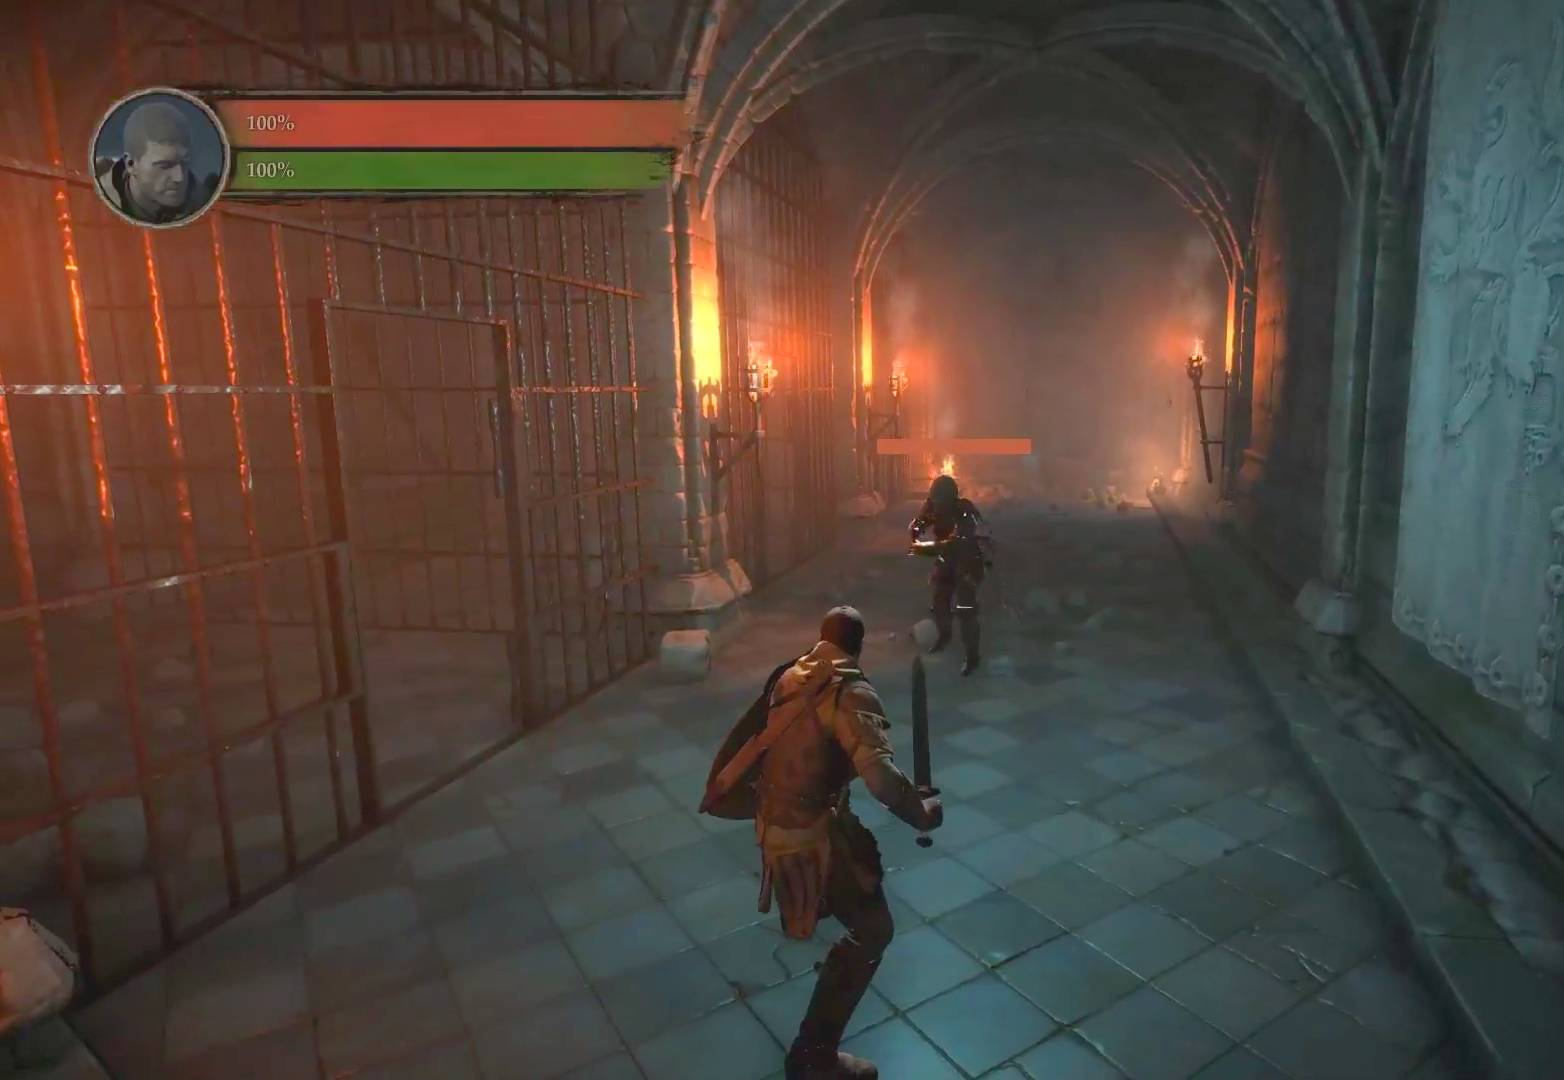
\includegraphics[width=26em]{figures/fig-bright-souls.jpg}
    \end{center}
    \legend{Source: Screen capture performed by the authors on a Microsoft Windows system.}
    \label{fig:ex1}
\end{figure}

To replicate the scenario of a successful commercial game, we look at how the problem of adaptive difficulty  is handled in multiple commercial games. Then, we analyze in depth the aspects that contribute to the difficulty of \emph{Dark Souls}, and attempt to replicate them in a simplified implementation. We compare the implementation of our solution to the original game, and outline the gameplay features that constitute the \emph{Souls}-like experience.

We propose a possible method for the design, implementation and usage of AGT as means of enhancing player experience. We compare the results in presence and absence of AGT, using as parameter a user evaluation on their perceived experience for each scenario and performance analysis based on gameplay data.

% ==========================================================
% Summary of each chapter
% ==========================================================

\section{Structure of this Work}

% Related work

% Analysis of Object of Study

% Implementation and Design

% Experiment Methodology and Results

% Discussion

% Conclusion